\chapter{Background} \label{c:Background}
The goal we are striving for is to animate human-like characters. In order to narrow it down even further we concentrate on the behaviour of the flesh of the character. 
For understanding the thematics of simulating human-like flesh it is necessary to have a basic mathematical background and knowledge of continuum mechanics. The goal of this chapter is to deliver an understanding in the topics mentioned.


\section{Notation and Convention}
At first we will declare the notation used in this thesis to avoid misunderstandings. We will use the common notation used in continuum mechanics taken from the book \textit{Continuum Mechanics} \cite{Spencer1980}. Additionally we will include some more specific declarations formulated and used in the paper \textit{Stable Neo-Hookean Flesh Simulation} \cite{Smith:2018:SNF:3191713.3180491}. 


\subsection{General Notation}
Scalars are represented by regular, normal-weight variables such as $a$ whereas 
tensors and matrices are represented by upper-case bold letters as for example $\textbf{A}$. Vectors will be denoted by bold lower-case variables like $\textbf{a}$. 


\subsection{Tensor Notation}
Furthermore we will use the tensor notation used in the paper \textit{Stable Neo-Hookean Flesh Simulation}. They decided to to define vectorization vec(.) as column-wise flattening of a matrix into a vector (\cite{Smith:2018:SNF:3191713.3180491}, 12:5) similar to Golub and Van Loan (2012) \cite{golub2012matrix}.

In order to indicate that we are dealing with a vectorized matrix we will use the symbol $\check{.}$ as shown in the following equation:

\[
\textbf{A} = \begin{bmatrix} a & c \\ b & d \end{bmatrix} \qquad \operatorname{vec}(\textbf{A}) = \boldsymbol{\check{a}} = \begin{bmatrix} a \\ b \\ c \\ d \end{bmatrix}.
\]

Additionally we will have to deal with $4^{th}$ order tensors in a form of matrix-of-matrices. These matrices are denoted by using blackboard bold:

\[
\mathbb{A} = 
\left[\begin{array}{cc}{\begin{bmatrix} a & c \\ b & d \end{bmatrix}} & {\begin{bmatrix} a & c \\ b & d \end{bmatrix}} \\ {\begin{bmatrix} a & c \\ b & d \end{bmatrix}} & {\begin{bmatrix} a & c \\ b & d \end{bmatrix}}\end{array}\right]
=
\left[\begin{array}{cc}{\left[\mathbf{A}_{00}\right]} & {\left[\mathbf{A}_{01}\right]} \\ {\left[\mathbf{A}_{10}\right]} & {\left[\mathbf{A}_{11}\right]}\end{array}\right]
\]

If we now vectorize $\mathbb{A}$ we receive the form described in the following line:

\[
\mathbb{A} = \operatorname{vec}(\mathbb{A})=\left[\operatorname{vec}\left(\mathrm{A}_{00}\right)\left|\operatorname{vec}\left(\mathrm{A}_{10}\right)\right| \operatorname{vec}\left(\mathrm{A}_{01}\right) | \operatorname{vec}\left(\mathrm{A}_{11}\right)\right]
\]

This term above is equivalent to the notation described here:

\[
\mathbb{A}=\left[\begin{array}{llll}{a} & {e} & {i} & {m} \\ {b} & {f} & {j} & {n} \\ {c} & {g} & {k} & {o} \\ {d} & {h} & {l} & {p}\end{array}\right] 
=\boldsymbol{\check{A}}
\]

The advantage of this form is that we can write several expressions as a cross product. We will need this property later to simplify complicated expressions and calculations.


\subsection{Summary}
A quick overview of the notation used so far:

\begin{addmargin}[1cm]{1cm}
a: Scalar \\
\textbf{A}: Matrix or tensor \\
\textbf{a}: Vector \\
vec(\textbf{A}) = $\boldsymbol{\check{a}}$: Vectorized matrix \\
$\mathbb{A} = \boldsymbol{\check{A}}$: matrix-of-matrices
\end{addmargin}

\todoredefined[inline]{
TODO: Check if all notations are declared when adding something.
}



\section{Mathematical Background}
Since mathematics play an important role in our field of interest we need to build a solid background before we go further into more complex calculations. This chapter should cover all the important concepts used later in the calculations. A basic understanding of linear algebra is assumed.


\subsection{Matrices}
At first we will discuss the physical or geometrical meaning of some common matrix properties.


\subsection{Singular Value Decomposition}

The singular value decomposition (SVD) will play an important role in formulating the deformation gradient. It is important for our application since it represents the best possible approximation of a given matrix by a matrix of low rank. This approximation can be looked at as a compression of the data given (\cite{LiesenMehrmann2015}, S. 295).

\begin{definition}[\textbf{Singular Values}]
The singular values of a matrix A $\in$ $\mathbb{R}^{m x n}$ are the square roots of the eigenvalues of $AA^{\mathrm{T}}$.
\end{definition}

The theorem of the singular value decomposition tells us that we can factor every m-by-n matrix into one orthogonal m-by-m, one diagonal m-by-n and one orthogonal n-by-n matrix. More formally:

\begin{theorem}[\textbf{The SVD Theorem}]
Let A $\in$ $\mathbb{R}^{m x n}$ be a matrix having r positive singular values, m $\geq$ n. Then there exist orthogonal matrices U $\in$ $\mathbb{R}^{m x m}$, V $\in$ $\mathbb{R}^{n x n}$ and a diagonal matrix $\tilde{\Sigma}$ $\in$ $\mathbb{R}^{m x n}$ such that

\[
\begin{array}{l}{A=U \tilde{\Sigma} V^{\mathrm{T}}} \\ {\tilde{\Sigma}=\left[\begin{array}{ll}{\Sigma} & {0} \\ {0} & {0}\end{array}\right]}\end{array}
\]

where $\Sigma$ = diag ($\sigma$1, $\sigma$2, . . . , $\sigma$r), and $\sigma$1 $\geq$ $\sigma$2 $\geq$ · · · $\geq$ $\sigma$r $>$ 0 are the positive singular values of A.

\end{theorem}
Reference: \cite{ford2014numerical}, chap. 15

\todoredefined[inline]{
TODO: Check reference. Make paragraphs work together. Add examples.
}


\subsection{Polar Decomposition}


\todoredefined[inline]{
TODO: Complete this section. Add lemmas and theorems used afterwards in the calculations. Possible adjustments may come at the end.
}



\section{Continuum Mechanics}
In this section we will give a broad introduction into the field of Continuum Mechanics. In Continuum Mechanics we are less interested in small particles like atoms or molecules of an object but rather concentrate on pieces of matter which are in comparison very large. We are therefore concerned with the mechanical behavior of solids and fluids on the macroscopic scale (\cite{Spencer1980}, p. 1).


\section{Deformation}
When applying a force over an object naturally the object itself undergoes a deformation. In the following we will be consistent with most previous literature in continuum mechanics and use the term strain as a measure of deformation and stress as the force per unit area.

\begin{addmargin}[2cm]{2cm}
\textit{Strain = measure of deformation}  \\
\textit{Stress = force per unit area} 
\end{addmargin}


\todoredefined[inline]{
TODO: Decide whether to include the above paragraph and how to connect it better to the paper.
}


Now let us have a look at a deformation in a rather mathematical sense. Graphically we can imagine a deformation with the help of a two dimensional deformation map as shown in Fig. \ref{fig:deformationmap}. Here we have on the left side an ellipse that represents an object or material in its rest state. A function $\phi$ maps this rest state of the ellipse to a deformed state shown in Fig. \ref{fig:deformationmap} on the right side. Mathematically spoken this means that we can map each point of a chosen object from its rest state to a deformed one.

\begin{figure}[!htbp]
	\centering
	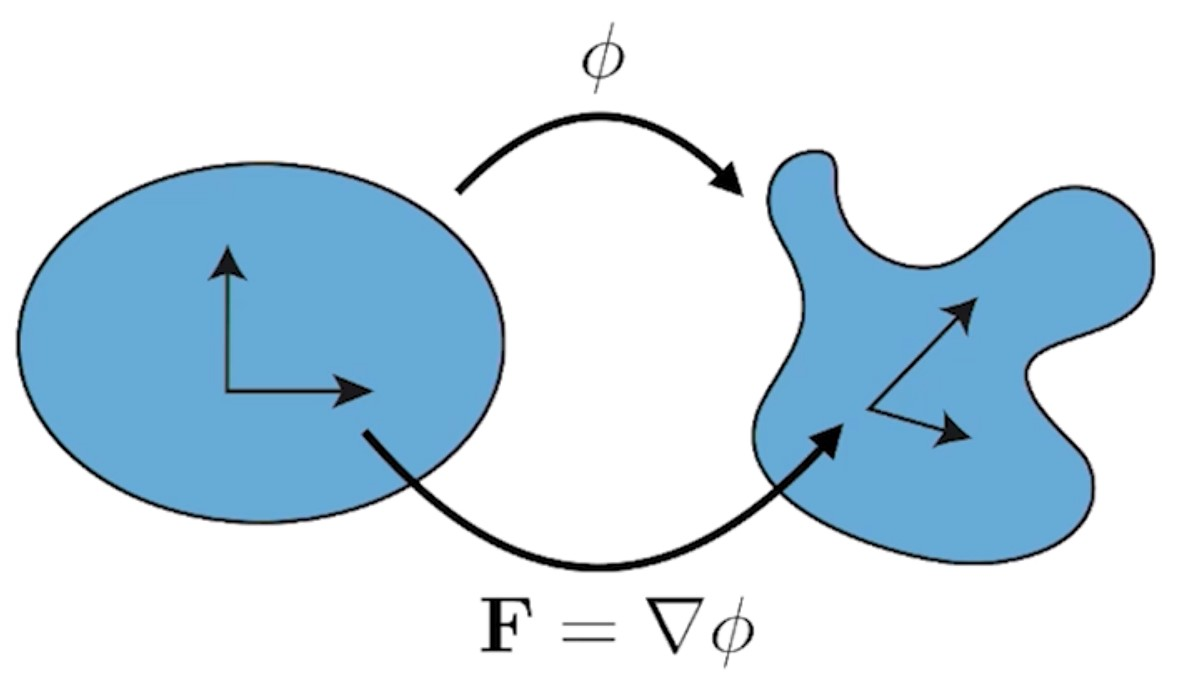
\includegraphics[width=0.5\textwidth]{resources/deformation_map}
	\caption{Deformation Map {\cite{STREAM2018}}}
	\label{fig:deformationmap}
\end{figure}

In conclusion the function $\phi$ describes our deformation. If we derive $\phi$ we can calculate the deformation gradient \textbf{F} which serves as a measure of the deformation in the following sense: 

\[
\begin{array}{l}
{\text { Deformation gradient: }} {\mathbf{F}=\operatorname{\nabla} \phi}
\\
{\text { Length changes: }} {\qquad I_{C}=\operatorname{tr}\left(\mathbf{F}^{T} \mathbf{F}\right)} 
\\ 
{\text { Volume changes: }} {\qquad J=\operatorname{det}(\mathbf{F})}\end{array}
\]

\todoredefined[inline]{
TODO: Adjust so the equal sign is at the same place in each column. Explain strain and stress and their meaning for later use in material constants (not explained in paper).
}


\subsection{Deformation Gradient}
The deformation gradient \textbf{F} offers us as said previously a measurement of the deformation. With its help we can amongst other things calculate the volume and length change an object undergoes during a deformation. For our needs we define the deformation gradient exactely as the authors of the paper \cite{Smith:2018:SNF:3191713.3180491} did:

\[
\textbf{F} = \left[ \,f_0\, \bigg| \,f_1\, \bigg| \,f_2\, \right] = \begin{bmatrix} f_0 & f_3 & f_6 \\ f_1 & f_4 & f_7 \\ f_2 & f_5 & f_8 \end{bmatrix}
\]


\todoredefined[inline]{
TODO: Add some examples. Already include definitions of the paper?
\\ Some more sources:
\\ http://www.continuummechanics.org/deformationgradient.html
}

\subsection{Polar Decomposition of the Deformation Gradient}
With the help of mathematics we can decompose the deformation gradient in the following form:

\[
F = R S
\]




\subsection{Material Constants}
When we look at a deformation of an object we need to consider the material the object consists of. A material can be very stiff like steel or easily deformable ones like robber. 

The two constants $\mu$ and $\lambda$ that are crucial for us are called \textit{Lamé Parameters}. With the help of these two constants we can calculate the \textit{Poisson's Ratio}:

\[ \sigma =  \frac{\lambda}{2(\lambda + \mu)} \in [-1, 0.5] \]

The poisson's ratio is of importance for us because it characterizes the materials resistance to volume change. Usually the poisson's ratio of a material is positive. A negative value would mean that the material becomes wider in the cross section when it is stretched. This behaviour is very uncommon in nature. Here are some examples of the poisson's ratio of common materials:

\begin{table}[h!]
\centering
    \begin{tabular}{ | l | l |}
    \hline
    Material & Poisson's ratio \\ \hline
    rubber & 0.4999 \\ \hline
    titanium & 0.265-0.34 \\ \hline
    glass & 0.18–0.3 \\ \hline
    cork & 0.0 \\ \hline
    \end{tabular}
    \caption{Different materials with their poisson's ratio}
\label{table:1}
\end{table}


For the simulation of human-like flesh we have to choose a poisson's ratio that is almost 0.5 in order to get realistic results.
\\ 

\todoredefined[inline]{
TODO: Add some examples and images. Explain poisson's ratio a bit better. Why must poisson's ratio be 0.5? Add some references. Make table more beautiful. Add reference to table, now it is wikipedia (https://en.wikipedia.org/wiki/Poisson%27s_ratio).
\\
Further reading: http://silver.neep.wisc.edu/~lakes/PoissonIntro.html
}



\subsection{Deformation Energy}
In order to get a convincing simulation of high quality we must choose an appropriate energy. In the case of modelling deformations on human-like characters we have to choose an elastic energy. The key property that makes an energy elastic is that if all the forces that are applied over an object add up to zero the object must come back into its rest shape.
\\
The energy then has to be minimized in order to get the results we want.

\begin{definition}
  This is a definition.
\end{definition}


\todoredefined[inline]{
TODO: Add some exaples and visualisations. What exactly is it and what role does it play in a deformation process? Hyperelastic energy, connect with paper.
\\ To include: Piola-Kirchhoff Stress, Cauchy Green invariant, polar decomposition, cauchy green tensor
}





